\documentclass[aspectratio=169]{beamer}

% Shared Beamer settings for Applied Machine Learning lectures (UPES).
% Keep this file free of \documentclass to allow reuse via \input.

% Allow lecture sources to use shared theme/assets without copying them into each lecture folder.
% NOTE: These paths are relative to `Unit-xx/Lecture-yy/latex/` (and `Lab/Experiment-xx/latex/`).
\makeatletter
\def\input@path{{../../../_shared/}{../../../_shared/UPES-Beamer-Theme/}}
\makeatother

\usetheme{UPES}
\setbeamertemplate{navigation symbols}{}

\usepackage{amsmath}
\usepackage{amssymb}
\usepackage{booktabs}
\usepackage{graphicx}
\usepackage{hyperref}
\usepackage{xcolor}
\usepackage{listings}

% Code listings (Python-oriented for this subject).
\lstset{
  language=Python,
  basicstyle=\ttfamily\small,
  keywordstyle=\color{blue},
  commentstyle=\color{gray},
  stringstyle=\color{teal},
  showstringspaces=false,
  columns=fullflexible,
  breaklines=true
}

\usepackage{tikz}
\usetikzlibrary{arrows.meta,positioning,shapes.geometric,calc,fit,backgrounds}

% Per-slide source line (references shown on the slide itself).
\newcommand{\slidesources}[1]{%
  \vfill
  {\tiny\color{gray}\raggedright\sloppy\parbox{\linewidth}{Sources: #1}\par}%
}

% Unit-wise source strings for this subject (used by slides/notes).
% Path is relative to the lecture `latex/` folder (the compilation CWD).
% Source strings for Applied Machine Learning (CSAI2017P) — used by slides + notes.
% Prescribed texts and reference books are taken from the course syllabus.
% Support texts are the author-hosted open-access editions:
%   statlearning.com            (ISL with Python)
%   probml.github.io/pml-book   (Murphy, Probabilistic Machine Learning)
%   d2l.ai                      (Dive into Deep Learning)
%   mml-book.github.io          (Mathematics for Machine Learning)

\newcommand{\AMLRepoURL}{https://github.com/tali7c/Applied-Machine-Learning}

% --- prescribed -------------------------------------------------------------
\newcommand{\AMLPrescribed}{%
M\"uller and Guido, \textit{Introduction to Machine Learning with Python}, O'Reilly, 2016.;%
Bishop, \textit{Pattern Recognition and Machine Learning}, Springer, 2006.;%
Murphy, \textit{Machine Learning: A Probabilistic Perspective}, MIT Press, 2012.;%
Han, Kamber and Pei, \textit{Data Mining: Concepts and Techniques} (3e), Morgan Kaufmann, 2012.%
}

% --- unit-wise ---------------------------------------------------------------
\newcommand{\AMLUnitISources}{%
M\"uller and Guido, \textit{Introduction to Machine Learning with Python}, Ch. 1.;%
Bishop, \textit{Pattern Recognition and Machine Learning}, Ch. 1.;%
Murphy, \textit{Probabilistic Machine Learning: An Introduction}, MIT Press, 2022, Ch. 1.;%
Mitchell, \textit{Machine Learning}, McGraw Hill, 1997, Ch. 1.;%
Scikit-learn documentation, accessed 2026-08-04.%
}

\newcommand{\AMLUnitIISources}{%
Bishop, \textit{Pattern Recognition and Machine Learning}, \S1.5, \S4.3, \S7.1.;%
Zhang, Lipton, Li and Smola, \textit{Dive into Deep Learning}, \S3.4.;%
Shalev-Shwartz and Ben-David, \textit{Understanding Machine Learning}, Ch. 15.;%
Murphy, \textit{Probabilistic Machine Learning: An Introduction}, Ch. 5.%
}

\newcommand{\AMLUnitIIISources}{%
Zhang, Lipton, Li and Smola, \textit{Dive into Deep Learning}, Ch. 12 (Optimization Algorithms).;%
Deisenroth, Faisal and Ong, \textit{Mathematics for Machine Learning}, Ch. 7.;%
Kingma and Ba, ``Adam: A Method for Stochastic Optimization,'' ICLR 2015.;%
Ruder, ``An overview of gradient descent optimization algorithms,'' arXiv:1609.04747, 2016.%
}

\newcommand{\AMLUnitIVSources}{%
Han, Kamber and Pei, \textit{Data Mining: Concepts and Techniques} (3e), Ch. 3.;%
M\"uller and Guido, \textit{Introduction to Machine Learning with Python}, Ch. 3--4.;%
James, Witten, Hastie, Tibshirani and Taylor, \textit{An Introduction to Statistical Learning with Python}, Ch. 5--6, 12.;%
Scikit-learn documentation (preprocessing, model selection), accessed 2026-08-04.%
}

\newcommand{\AMLUnitVSources}{%
James et al., \textit{An Introduction to Statistical Learning with Python}, Ch. 3--6.;%
Bishop, \textit{Pattern Recognition and Machine Learning}, Ch. 3.;%
Deisenroth, Faisal and Ong, \textit{Mathematics for Machine Learning}, Ch. 9.;%
M\"uller and Guido, \textit{Introduction to Machine Learning with Python}, \S2.3.%
}

\newcommand{\AMLUnitVISources}{%
Han, Kamber and Pei, \textit{Data Mining: Concepts and Techniques} (3e), Ch. 8--9.;%
James et al., \textit{An Introduction to Statistical Learning with Python}, Ch. 8--9.;%
Bishop, \textit{Pattern Recognition and Machine Learning}, Ch. 4--5, 7, 14.;%
Zhang et al., \textit{Dive into Deep Learning}, Ch. 5.%
}

\newcommand{\AMLUnitVIISources}{%
Han, Kamber and Pei, \textit{Data Mining: Concepts and Techniques} (3e), Ch. 10.;%
James et al., \textit{An Introduction to Statistical Learning with Python}, Ch. 12.;%
M\"uller and Guido, \textit{Introduction to Machine Learning with Python}, \S3.5.;%
Ester, Kriegel, Sander and Xu, ``A density-based algorithm for discovering clusters (DBSCAN),'' KDD 1996.%
}

\newcommand{\AMLLabSources}{%
M\"uller and Guido, \textit{Introduction to Machine Learning with Python}, companion notebooks.;%
McKinney, \textit{Python for Data Analysis} (3e), O'Reilly, 2022.;%
Scikit-learn user guide, accessed 2026-08-04.;%
Matplotlib and Seaborn documentation, accessed 2026-08-04.%
}



\graphicspath{{../figures/}{../images/}{../../../_shared/}{../../../_shared/UPES-Beamer-Theme/}}

\title[Applied Machine Learning]{Applied Machine Learning}
\subtitle{Unit 05 -- Lecture 11: Multiple Linear Regression}
\author{Tofik Ali}
\institute{School of Computer Science, UPES Dehradun}
\date{Autumn 2026}

% ---- a compact "output" block so code and its result sit together ----------
\lstdefinestyle{outblk}{
  basicstyle=\ttfamily\scriptsize\color{black!75},
  backgroundcolor=\color{black!5}, frame=leftline, framerule=2pt,
  rulecolor=\color{black!30}, breaklines=true, columns=fullflexible,
  keepspaces=true,   % several outputs below are aligned tables
  language={},       % printed output is not Python: do not syntax-highlight it
  xleftmargin=4pt, aboveskip=1pt, belowskip=1pt, literate={-}{{-}}1}
\lstnewenvironment{outblk}{\lstset{style=outblk}}{}

\newcommand{\Xt}{X^{\!\top}}

\begin{document}

\UPESCoverFrame
\setcounter{framenumber}{0}

\begin{frame}
  \titlepage
  \begin{center}
    \footnotesize Building, deriving, interpreting and validating a model with
    many predictors\\[0.25em]
    \footnotesize Topic focus: \textbf{a coefficient is a conditional
    statement, not a fact about a column}\\[0.25em]
    \footnotesize Repository: \texttt{\AMLRepoURL}
  \end{center}
  \slidesources{\AMLUnitVSources}
\end{frame}

\begin{frame}{Quick Links}
  \centering
  \hyperlink{sec:model}{\beamerbutton{The model}}\hspace{0.4em}
  \hyperlink{sec:derive}{\beamerbutton{The derivation}}\hspace{0.4em}
  \hyperlink{sec:hand}{\beamerbutton{By hand}}\hspace{0.4em}
  \hyperlink{sec:interp}{\beamerbutton{Interpretation}}\hspace{0.4em}
  \hyperlink{sec:std}{\beamerbutton{Standardized}}\hspace{0.4em}
  \hyperlink{sec:mc}{\beamerbutton{Collinearity}}\hspace{0.4em}
  \hyperlink{sec:missing}{\beamerbutton{Missing data}}\hspace{0.4em}
  \hyperlink{sec:valid}{\beamerbutton{Validation}}\hspace{0.4em}
  \hyperlink{sec:summary}{\beamerbutton{Summary}}
\end{frame}

\begin{frame}{Agenda}
  \tableofcontents
\end{frame}

\begin{frame}[shrink=6]{How this lecture works}
  \begin{columns}[T]
    \begin{column}{0.48\textwidth}
      \begin{block}{Every idea appears twice}
        \begin{enumerate}
          \item \textbf{By hand} --- five flats, two predictors, a
            $3\times3$ matrix inverted with cofactors. Integer arithmetic
            throughout; nothing rounds.
          \item \textbf{In code} --- the same quantities on $442$ diabetes
            patients, so you see that \texttt{LinearRegression} solves
            exactly that system and nothing more.
        \end{enumerate}
      \end{block}
    \end{column}
    \begin{column}{0.48\textwidth}
      \begin{alertblock}{Commit before you look}
        Four slides ask you to predict a number before it is revealed. Write
        your guess down. Being wrong on paper is how the idea sticks.
      \end{alertblock}
    \end{column}
  \end{columns}
  \vspace{0.4em}
  \begin{center}
    \small The centrepiece is \textbf{a predictor whose coefficient is
    $+0.47$ on its own and $-1.09$ once its neighbours join the model}.
    Everything after it exists to explain why that is not a bug.
  \end{center}
\end{frame}

\begin{frame}[shrink=5]{Where we are}
  \begin{columns}[T]
    \begin{column}{0.47\textwidth}
      \begin{block}{You already have the one-predictor case}
        $\hat y = b_0 + b_1 x$, least squares, the two normal equations,
        $R^2$, and maximum likelihood under Gaussian noise. Nothing in this
        lecture replaces any of it.
      \end{block}
      \begin{block}{Real tables have many columns}
        A patient has ten measurements, a flat has five attributes, a loan
        application has forty. Fitting them one at a time answers the wrong
        question.
      \end{block}
    \end{column}
    \begin{column}{0.49\textwidth}
      \begin{exampleblock}{Today's five questions}
        How do we write the model for $p$ predictors? Where does
        $\hat\beta = (\Xt X)^{-1}\Xt y$ come from, and when does it fail?
        What does a coefficient \emph{mean}? Which coefficients can be
        compared? And how do we know the model is any good?
      \end{exampleblock}
      \begin{alertblock}{One sentence to carry throughout}
        \small A multiple-regression coefficient is the effect of a predictor
        \textbf{holding the others fixed}. Change the others and you change
        the coefficient.
      \end{alertblock}
    \end{column}
  \end{columns}
\end{frame}

\begin{frame}[shrink=5]{One seed --- and one thing we deliberately do not fix}
  \begin{columns}[T]
    \begin{column}{0.48\textwidth}
      \begin{block}{Seed $0$, for everything arbitrary}
        \small Splits, the eight-patient subset, the simulated missing cells,
        the imputer, the junk columns, the collinear pair. The data itself
        (\texttt{load\_diabetes(scaled=False)}, \texttt{load\_wine}) is
        bundled and never generated.
      \end{block}
    \end{column}
    \begin{column}{0.48\textwidth}
      \begin{alertblock}{The bootstrap is a \emph{sweep}}
        \small $2000$ resamples, \texttt{range(0, 2000)}. \textbf{The spread
        across them is the whole result} --- it is how we show a coefficient
        is not reportable. Collapsing it to one seed would delete the
        demonstration.
      \end{alertblock}
    \end{column}
  \end{columns}
  \vspace{0.4em}
  \begin{exampleblock}{The distinction is worth learning}
    \centering\small
    A seed you picked arbitrarily should be fixed and stated. A set of seeds
    you are \emph{deliberately varying} is an experiment, and its variability
    is data. Every number in this deck reproduces exactly.
  \end{exampleblock}
\end{frame}

% =====================================================================
\section[Model]{The model and the design matrix}
\label{sec:model}

\begin{frame}[shrink=6]{From one predictor to $p$}
  \begin{exampleblock}{}
    \centering\large
    $y_i = \beta_0 + \beta_1 x_{i1} + \beta_2 x_{i2} + \dots +
     \beta_p x_{ip} + \varepsilon_i,
     \qquad i = 1,\dots,n$
  \end{exampleblock}
  \vspace{0.3em}
  \begin{columns}[T]
    \begin{column}{0.52\textwidth}
      \begin{block}{Stack the rows and it is one equation}
        \[
          \underbrace{y}_{n\times 1} =
          \underbrace{X}_{n\times(p+1)}\,
          \underbrace{\beta}_{(p+1)\times 1} + \varepsilon,
        \]
        with a leading column of ones in $X$ so that $\beta_0$ is an ordinary
        coefficient and needs no special treatment.
      \end{block}
    \end{column}
    \begin{column}{0.44\textwidth}
      \begin{block}{What ``linear'' means}
        \small Linear \textbf{in the parameters}, not in the predictors.
        $y = \beta_0 + \beta_1 x + \beta_2 x^2$ is a multiple linear
        regression with $x_2 = x^2$. $y = \beta_0 x^{\beta_1}$ is not.
      \end{block}
      \begin{alertblock}{The geometry}
        \small One predictor fits a \emph{line} in the plane. Two fit a
        \emph{plane} in three dimensions. $p$ fit a $p$-dimensional
        \textbf{hyperplane}.
      \end{alertblock}
    \end{column}
  \end{columns}
\end{frame}

\begin{frame}[shrink=8]{By hand: five flats, two predictors}
  Price in lakh of rupees. $x_1$ is the number of bedrooms; $x_2$ is the floor
  area in units of $50\,\mathrm{m}^2$.
  \begin{center}\small
  \begin{tabular}{@{}lrrrrr@{}}
    \toprule
    flat & A & B & C & D & E\\
    \midrule
    bedrooms $x_1$ & $1$ & $2$ & $3$ & $4$ & $5$\\
    area $x_2$ & $2$ & $3$ & $4$ & $3$ & $4$\\
    \midrule
    \textbf{price} $y$ & $8$ & $13$ & $15$ & $11$ & $12$\\
    \bottomrule
  \end{tabular}
  \end{center}
  \vspace{0.2em}
  \[
    X = \begin{pmatrix}
      1 & 1 & 2\\ 1 & 2 & 3\\ 1 & 3 & 4\\ 1 & 4 & 3\\ 1 & 5 & 4
    \end{pmatrix},
    \qquad
    y = \begin{pmatrix} 8\\13\\15\\11\\12 \end{pmatrix},
    \qquad
    n = 5,\quad p = 2 .
  \]
  \begin{block}{Look at flats B and D before we compute anything}
    \small Both are $150\,\mathrm{m}^2$. B has $2$ bedrooms and costs $13$;
    D has $4$ and costs $11$. \textbf{At a fixed area, an extra bedroom is
    worth $-1$ lakh.} Hold that thought.
  \end{block}
\end{frame}

% =====================================================================
\section[Derivation]{Deriving \texorpdfstring{$\hat\beta = (\Xt X)^{-1}\Xt y$}{beta-hat = (X\textquotesingle X)\textasciicircum-1 X\textquotesingle y}}
\label{sec:derive}

\begin{frame}[shrink=6]{The objective, written once}
  Least squares chooses $b$ to minimise the sum of squared residuals:
  \[
    S(b) \;=\; \sum_{i=1}^{n}\bigl(y_i - x_i^{\!\top} b\bigr)^2
         \;=\; (y - Xb)^{\!\top}(y - Xb).
  \]
  Expand, using $b^{\!\top}\Xt y = y^{\!\top} X b$ (both are $1\times1$, so
  each is its own transpose):
  \begin{equation*}
    S(b) = y^{\!\top}y \;-\; 2\,b^{\!\top}\Xt y \;+\; b^{\!\top}\Xt X\,b .
  \end{equation*}
  \begin{block}{Three terms, three shapes}
    \small $y^{\!\top}y$ is a constant. $-2b^{\!\top}\Xt y$ is
    \textbf{linear} in $b$. $b^{\!\top}\Xt X b$ is a \textbf{quadratic form},
    and $\Xt X$ is symmetric and positive semi-definite --- which is exactly
    why this problem has a minimum and not a saddle.
  \end{block}
\end{frame}

\begin{frame}[shrink=6]{Two facts of matrix calculus, and that is all you need}
  \begin{columns}[T]
    \begin{column}{0.48\textwidth}
      \begin{block}{Linear term}
        \[ \frac{\partial}{\partial b}\bigl(b^{\!\top}c\bigr) = c \]
        \small Check componentwise: $b^{\!\top}c = \sum_j b_j c_j$, so
        $\partial/\partial b_k = c_k$.
      \end{block}
    \end{column}
    \begin{column}{0.48\textwidth}
      \begin{block}{Quadratic form, $A$ symmetric}
        \[ \frac{\partial}{\partial b}\bigl(b^{\!\top}Ab\bigr) = 2Ab \]
        \small Check componentwise:
        $b^{\!\top}Ab = \sum_j\sum_k b_j A_{jk} b_k$, so
        $\partial/\partial b_m = 2\sum_k A_{mk}b_k$.
      \end{block}
    \end{column}
  \end{columns}
  \vspace{0.3em}
  Apply both to $S(b) = y^{\!\top}y - 2b^{\!\top}\Xt y + b^{\!\top}\Xt X b$:
  \[
    \nabla S(b) \;=\; -2\,\Xt y \;+\; 2\,\Xt X\,b .
  \]
  \begin{alertblock}{And the second derivative}
    \small $\nabla^2 S(b) = 2\,\Xt X \succeq 0$, so every stationary point is
    a \textbf{global} minimum. There are no local minima to worry about ---
    which is why regression is not an optimisation problem in the way that
    training a network is.
  \end{alertblock}
\end{frame}

\begin{frame}[shrink=6]{Set the gradient to zero: the normal equations}
  \[
    -2\,\Xt y + 2\,\Xt X\,\hat\beta = 0
    \qquad\Longleftrightarrow\qquad
    \boxed{\;\Xt X\,\hat\beta = \Xt y\;}
  \]
  \vspace{-0.4em}
  \[
    \text{and if } \Xt X \text{ is invertible,}\qquad
    \boxed{\;\hat\beta = (\Xt X)^{-1}\,\Xt y\;}
  \]
  \begin{columns}[T]
    \begin{column}{0.48\textwidth}
      \begin{block}{This is the simple case, generalised}
        \small With one predictor,
        $\Xt X = \left(\begin{smallmatrix} n & \sum x\\
        \sum x & \sum x^2\end{smallmatrix}\right)$ and
        $\Xt y = \left(\begin{smallmatrix}\sum y\\
        \sum xy\end{smallmatrix}\right)$. Solving the
        $2\times2$ system gives $b_1 = S_{xy}/S_{xx}$ and
        $b_0 = \bar y - b_1\bar x$. \textbf{Same equations.}
      \end{block}
    \end{column}
    \begin{column}{0.48\textwidth}
      \begin{alertblock}{Read the boxed line as a warning}
        \small The formula is only a formula \emph{if} $\Xt X$ can be
        inverted. The whole of the next slide is about when it cannot ---
        and multicollinearity, later in the lecture, is the case where it
        \emph{barely} can.
      \end{alertblock}
    \end{column}
  \end{columns}
\end{frame}

\begin{frame}[shrink=6]{When is $\Xt X$ invertible?}
  \begin{block}{Proof of the equivalence, in three lines}
    \small
    Suppose $\Xt X v = 0$ for some $v \ne 0$. Then
    $v^{\!\top}\Xt X v = \|Xv\|^2 = 0$, so $Xv = 0$: the columns of $X$ are
    linearly dependent. Conversely if $Xv = 0$ then $\Xt X v = 0$. Hence
    \[
      \operatorname{null}(\Xt X) = \operatorname{null}(X),
      \qquad\text{so}\qquad
      \operatorname{rank}(\Xt X) = \operatorname{rank}(X).
    \]
    $\Xt X$ is $(p{+}1)\times(p{+}1)$, so it is invertible exactly when
    $\operatorname{rank}(X) = p+1$: \textbf{full column rank}.
  \end{block}
  \vspace{0.2em}
  \begin{columns}[T]
    \begin{column}{0.48\textwidth}
      \begin{alertblock}{Failure 1: perfect collinearity}
        \small One column is an exact linear combination of the others.
        Duplicated columns, a total and its parts, all $k$ dummies plus an
        intercept, the same quantity in two units.
      \end{alertblock}
    \end{column}
    \begin{column}{0.48\textwidth}
      \begin{alertblock}{Failure 2: $p+1 > n$}
        \small More parameters than rows. Then
        $\operatorname{rank}(X) \le n < p+1$ \textbf{whatever the numbers
        are}. Gene expression, text, any wide table.
      \end{alertblock}
    \end{column}
  \end{columns}
\end{frame}

\begin{frame}[shrink=6]{The same condition, seen geometrically}
  \begin{columns}[T]
    \begin{column}{0.52\textwidth}
      \begin{block}{What the normal equations say}
        Rearrange $\Xt X\hat\beta = \Xt y$:
        \[ \Xt(y - X\hat\beta) = \Xt e = 0 . \]
        \textbf{Every column of $X$ is orthogonal to the residual vector.}
        The fitted values $\hat y = X\hat\beta$ are the orthogonal projection
        of $y$ onto the column space of $X$, and $e$ is what is left over.
      \end{block}
      \begin{block}{The hat matrix}
        \small $\hat y = Hy$ with $H = X(\Xt X)^{-1}\Xt$. $H$ is symmetric,
        $H^2 = H$, and $\operatorname{tr}(H) = p+1$ --- the number of
        parameters. You will meet $H$ again in the diagnostics section.
      \end{block}
    \end{column}
    \begin{column}{0.44\textwidth}
      \begin{exampleblock}{Two consequences you can check on paper}
        \small Because the first column of $X$ is all ones,
        $\Xt e = 0$ forces $\sum_i e_i = 0$: \textbf{the residuals always sum
        to zero}. And because the $j$th column is $x_j$, it forces
        $\sum_i x_{ij}e_i = 0$: \textbf{the residuals are uncorrelated with
        every predictor, by construction}.
      \end{exampleblock}
      \begin{alertblock}{So do not be impressed}
        \small ``My residuals have mean zero and no correlation with the
        inputs'' is not evidence that the model is right. It is arithmetic.
      \end{alertblock}
    \end{column}
  \end{columns}
\end{frame}

\begin{frame}[fragile,shrink=8]{Failure 1 in code: an exact linear combination}
Add a third column $x_3 = x_1 + x_2$ to the five flats. Nothing is wrong with
the data; the \emph{matrix} is now rank deficient.
\begin{outblk}
shape (5, 4)  rank 3  (needs 4)
det(X'X) = 0.000000e+00
np.linalg.inv  ->  LinAlgError: Singular matrix
condition number of X'X: 7.692e+18
\end{outblk}
\onslide<2->
\begin{outblk}
LinearRegression still answers: [ 2. -2.  3.  1.]
a DIFFERENT coefficient vector: [ 2. -1.  4.  0.]
max |difference in predictions| 0.00e+00
\end{outblk}
\onslide<3->
\begin{alertblock}{The library did not raise, and its answer is not unique}
  \footnotesize \texttt{LinearRegression} calls \texttt{lstsq}, which returns
  the \emph{minimum-norm} solution instead of failing. Add $c$ to $b_1$ and
  $b_2$ and subtract $c$ from $b_3$ and the predictions do not change by
  $10^{-16}$. \textbf{The predictions are fine; the coefficients mean
  nothing.} This is the dummy variable trap of Lecture~6 in its general form.
\end{alertblock}
\end{frame}

\begin{frame}[fragile,shrink=8]{Failure 2 in code: more parameters than patients}
Take $8$ diabetes patients and all $10$ features.
\begin{outblk}
8 patients, 10 features + intercept -> X is (8, 11)
rank(X) = 8, so rank(X'X) = 8 but X'X is 11 x 11
np.linalg.inv  ->  LinAlgError: Singular matrix
lstsq minimum-norm solution ||b|| = 31.5783, SSE = 3.709e-24
add 100 * a null-space direction: ||b|| = 104.8675, SSE = 2.614e-23
\end{outblk}
\onslide<2->
\begin{center}\small
  Both vectors fit all eight rows \textbf{exactly}, and they are two of an
  infinite family: the null space of $X$ has dimension
  $11 - 8 = 3$, so you may move $\hat\beta$ anywhere in a $3$-dimensional
  affine set at zero cost.
\end{center}
\onslide<3->
\begin{alertblock}{This is the problem regularisation exists to solve}
  \footnotesize Ridge replaces $\Xt X$ by $\Xt X + \lambda I$, which is
  \emph{always} invertible for $\lambda > 0$, and picks one member of that
  family. That is the next lecture. \textbf{Note what the disease is: not
  ``too little signal'' but ``no unique answer''.}
\end{alertblock}
\end{frame}

% =====================================================================
\section[By hand]{The five flats, worked completely}
\label{sec:hand}

\begin{frame}[shrink=6]{Step 1: form $\Xt X$ and $\Xt y$}
  Every entry is a sum you can do in your head.
  \[
    \Xt X =
    \begin{pmatrix}
      n & \sum x_1 & \sum x_2\\
      \sum x_1 & \sum x_1^2 & \sum x_1x_2\\
      \sum x_2 & \sum x_1x_2 & \sum x_2^2
    \end{pmatrix}
    =
    \begin{pmatrix} 5 & 15 & 16\\ 15 & 55 & 52\\ 16 & 52 & 54 \end{pmatrix},
    \qquad
    \Xt y = \begin{pmatrix} 59\\ 183\\ 196 \end{pmatrix}.
  \]
  \begin{center}\small
  \begin{tabular}{@{}lrl@{}}
    \toprule
    $\sum x_1 = 1{+}2{+}3{+}4{+}5$ & $= 15$ & $\sum y = 8{+}13{+}15{+}11{+}12 = 59$\\
    $\sum x_1^2 = 1{+}4{+}9{+}16{+}25$ & $= 55$ & $\sum x_1 y = 8{+}26{+}45{+}44{+}60 = 183$\\
    $\sum x_1x_2 = 2{+}6{+}12{+}12{+}20$ & $= 52$ & $\sum x_2 y = 16{+}39{+}60{+}33{+}48 = 196$\\
    \bottomrule
  \end{tabular}
  \end{center}
  \begin{block}{$\Xt X$ is symmetric, and that is not a coincidence}
    \small $(\Xt X)^{\!\top} = \Xt X$ for any $X$ at all. So you only ever
    compute the upper triangle: six numbers here, not nine.
  \end{block}
\end{frame}

\begin{frame}[shrink=8]{Step 2: invert it with cofactors}
  For the symmetric matrix $M = \Xt X$, the cofactors along the first row are
  \[
    A_{11} = 55\cdot54 - 52^2 = 266,\quad
    A_{12} = -(15\cdot54 - 52\cdot16) = 22,\quad
    A_{13} = 15\cdot52 - 55\cdot16 = -100,
  \]
  \[
    \det M = 5(266) + 15(22) + 16(-100) = 1330 + 330 - 1600 = \mathbf{60}.
  \]
  The remaining cofactors are $A_{22} = 5\cdot54-16^2 = 14$,
  $A_{23} = -(5\cdot52-15\cdot16) = -20$, $A_{33} = 5\cdot55-15^2 = 50$, so
  \[
    (\Xt X)^{-1} = \frac{1}{60}
    \begin{pmatrix} 266 & 22 & -100\\ 22 & 14 & -20\\ -100 & -20 & 50
    \end{pmatrix}.
  \]
  \begin{alertblock}{$\det = 60$ is small relative to the entries}
    \small That is the first hint of what is coming: $x_1$ and $x_2$
    correlate at $+0.756$, so the matrix is closer to singular than its size
    suggests. Perfectly invertible here --- \emph{barely} invertible is the
    subject of the multicollinearity section.
  \end{alertblock}
\end{frame}

\begin{frame}[shrink=6]{Step 3: multiply, and read the answer}
  \[
    \hat\beta = (\Xt X)^{-1}\Xt y = \frac{1}{60}
    \begin{pmatrix} 266 & 22 & -100\\ 22 & 14 & -20\\ -100 & -20 & 50
    \end{pmatrix}
    \begin{pmatrix} 59\\183\\196 \end{pmatrix}
  \]
  \begin{center}\small
  \begin{tabular}{@{}ll@{}}
    \toprule
    $266(59) + 22(183) - 100(196) = 15694 + 4026 - 19600 = 120$ &
      $\Rightarrow\ b_0 = 120/60 = \mathbf{2}$\\
    $\phantom{2}22(59) + 14(183) - \phantom{1}20(196) = \phantom{1}1298 + 2562 - \phantom{1}3920 = -60$ &
      $\Rightarrow\ b_1 = -60/60 = \mathbf{-1}$\\
    $-100(59) - 20(183) + \phantom{1}50(196) = -5900 - 3660 + \phantom{1}9800 = 240$ &
      $\Rightarrow\ b_2 = 240/60 = \mathbf{4}$\\
    \bottomrule
  \end{tabular}
  \end{center}
  \begin{exampleblock}{}
    \centering\large
    $\hat y \;=\; 2 \;-\; 1\cdot x_1 \;+\; 4\cdot x_2$
  \end{exampleblock}
  \begin{center}\small
    \textbf{The bedroom coefficient is negative.} An extra $50\,\mathrm{m}^2$
    is worth $+4$ lakh; an extra bedroom \emph{in the same area} is worth
    $-1$ lakh --- which is exactly what flats B and D said before we started.
  \end{center}
\end{frame}

\begin{frame}[shrink=8]{Step 4: check it, the way the derivation tells you to}
  \begin{center}\small
  \begin{tabular}{@{}lrrrrr@{}}
    \toprule
    & A & B & C & D & E\\
    \midrule
    $\hat y = 2 - x_1 + 4x_2$ & $9$ & $12$ & $15$ & $10$ & $13$\\
    $y$ & $8$ & $13$ & $15$ & $11$ & $12$\\
    \textbf{residual} $e$ & $-1$ & $+1$ & $0$ & $+1$ & $-1$\\
    \bottomrule
  \end{tabular}
  \end{center}
  \vspace{0.2em}
  \[
    \textstyle\sum e_i = 0,\qquad
    \sum x_{1i}e_i = -1+2+0+4-5 = 0,\qquad
    \sum x_{2i}e_i = -2+3+0+3-4 = 0 .
  \]
  \begin{columns}[T]
    \begin{column}{0.48\textwidth}
      \begin{block}{Fit statistics}
        \small $\mathrm{SSE} = 1+1+0+1+1 = 4$. \\
        $\bar y = 11.8$, so
        $\mathrm{SST} = 26.8$.\\
        $R^2 = 1 - 4/26.8 = \mathbf{0.8507}$.\\
        $R^2_{\text{adj}} = 1 - \dfrac{4/2}{26.8/4} = \mathbf{0.7015}$.
      \end{block}
    \end{column}
    \begin{column}{0.48\textwidth}
      \begin{alertblock}{$\Xt e = 0$ is the check that matters}
        \small Those three zeros are the normal equations, read backwards.
        If your hand arithmetic gets $\hat\beta$ wrong, they will not come
        out --- so compute them every time. Two minutes of insurance.
      \end{alertblock}
    \end{column}
  \end{columns}
\end{frame}

\begin{frame}[fragile,shrink=6]{The same thing in code}
\begin{lstlisting}
X = np.c_[np.ones(5), x1, x2]
beta = np.linalg.inv(X.T @ X) @ (X.T @ y)          # by hand
lr = LinearRegression().fit(np.c_[x1, x2], y)      # by library
\end{lstlisting}
\begin{outblk}
X'X =
 [[ 5 15 16]
 [15 55 52]
 [16 52 54]]
X'y = [ 59 183 196]
det(X'X) = 60
60 * inv(X'X) =
 [[ 266.   22. -100.]
 [  22.   14.  -20.]
 [-100.  -20.   50.]]
beta = inv(X'X) X'y = [ 2. -1.  4.]
LinearRegression intercept 2.0000000000  coef [-1.  4.]
max |difference| 8.62e-14
\end{outblk}
\onslide<2->
\begin{center}\small
  \textbf{Every number in the hand calculation, to the last digit.} The
  $8.62\times10^{-14}$ is floating point, not disagreement. Note that
  \texttt{sklearn} does \emph{not} form the inverse --- it calls
  \texttt{scipy.linalg.lstsq}, which is slower to describe and far more
  numerically stable.
\end{center}
\end{frame}

\begin{frame}[fragile,shrink=8]{A shortcut worth knowing: centre first}
Subtract the column means. The intercept then separates out and you invert a
$2\times2$ instead of a $3\times3$:
\[
  \begin{pmatrix} S_{11} & S_{12}\\ S_{12} & S_{22}\end{pmatrix}
  \begin{pmatrix} b_1\\ b_2\end{pmatrix}
  = \begin{pmatrix} S_{1y}\\ S_{2y}\end{pmatrix},
  \qquad
  b_0 = \bar y - b_1\bar x_1 - b_2\bar x_2 .
\]
\begin{outblk}
centred cross-product matrix
 [[10.   4. ]
 [ 4.   2.8]]
det 12.0   inverse * 12 =
 [[ 2.8 -4. ]
 [-4.  10. ]]
X'y centred       [6.0 7.2]
slopes from the 2x2 system [-1.  4.]
intercept = ybar - b1*x1bar - b2*x2bar = 2.0
\end{outblk}
\onslide<2->
\begin{center}\small
  $b_1 = \dfrac{2.8(6.0) - 4(7.2)}{12} = \dfrac{-12}{12} = -1$,\quad
  $b_2 = \dfrac{-4(6.0) + 10(7.2)}{12} = \dfrac{48}{12} = 4$.
  \textbf{Two lines of arithmetic and the same answer.} This is the form to
  use in an examination.
\end{center}
\end{frame}

\begin{frame}[shrink=8]{Drawn: the marginal picture and the fitted plane}
  \begin{center}
    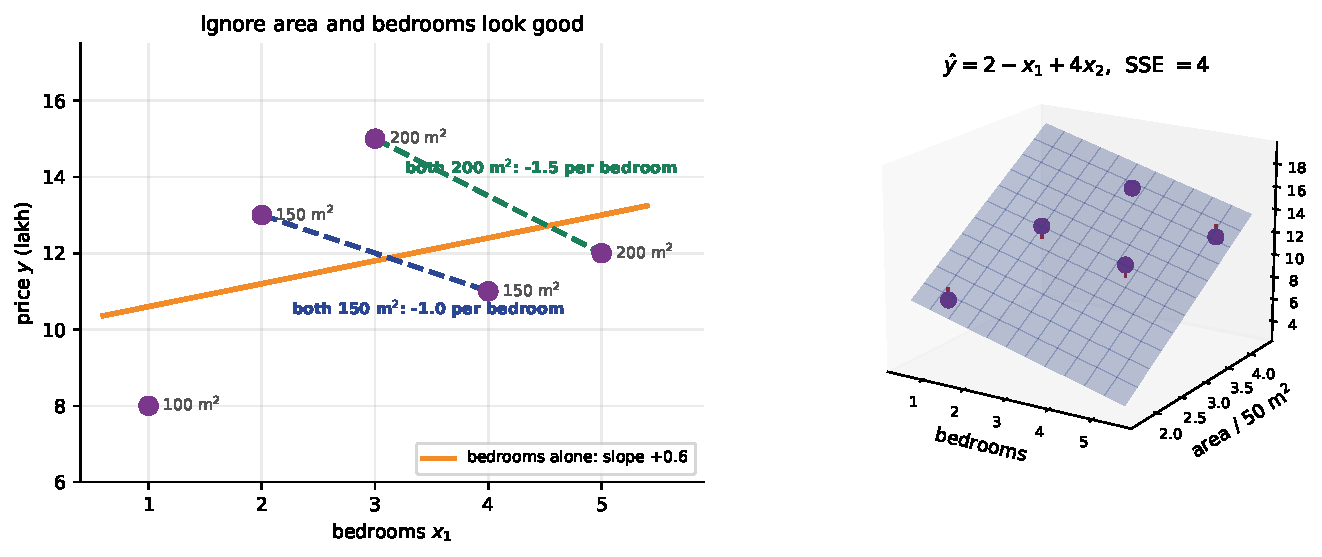
\includegraphics[width=0.88\textwidth]{hand.pdf}
  \end{center}
  \begin{center}\small
    Left: ignore area and bedrooms look good --- the orange line has slope
    $+0.6$. But join the two flats that share a floor area and the dashed
    segments go \emph{down}. Right: the fitted plane, with the five
    residuals drawn as vertical bars summing to $\mathrm{SSE} = 4$.
  \end{center}
\end{frame}

% =====================================================================
\section[Meaning]{What a coefficient means}
\label{sec:interp}

\begin{frame}[shrink=6]{``Holding the others fixed''}
  \begin{exampleblock}{}
    \centering
    $b_j$ is the change in $\hat y$ for a one-unit increase in $x_j$
    \textbf{when every other predictor in the model is held constant}.
  \end{exampleblock}
  \vspace{0.3em}
  \begin{columns}[T]
    \begin{column}{0.48\textwidth}
      \begin{block}{Three words that do all the work}
        \small \textbf{In the model.} Not ``in the world''. The clause names
        the other columns \emph{you happened to include}. Add a column,
        remove a column, and $b_j$ changes --- legitimately, because it is
        now answering a different question.
      \end{block}
    \end{column}
    \begin{column}{0.48\textwidth}
      \begin{block}{The flats again}
        \small $b_1 = -1$ does not say bedrooms make a flat cheaper. It says:
        among flats of the \emph{same area}, the one chopped into more
        bedrooms is worth less. Both statements can be true, and the data
        contain both.
      \end{block}
    \end{column}
  \end{columns}
  \vspace{0.2em}
  \begin{alertblock}{And the clause can be physically impossible}
    \small ``Holding total cholesterol fixed, LDL cholesterol has effect
    $b$'' describes an intervention nobody can perform. The number is still
    computable, and still means something --- but not what a headline would
    say it means.
  \end{alertblock}
\end{frame}

\begin{frame}[fragile,shrink=8]{Predict first \#1}
\texttt{load\_diabetes(scaled=False)}: $442$ patients, $10$ measurements in
their original units, target is disease progression after one year.

Regress the target on \texttt{s1}, total serum cholesterol, \textbf{on its
own}. The slope is $\mathbf{+0.4723}$ per mg/dl --- more cholesterol, worse
progression, as everyone expects.

\begin{center}
  \textbf{Now put the other nine measurements into the model.
  What happens to the \texttt{s1} coefficient?}
\end{center}
\vspace{0.2em}
\onslide<2->
\begin{outblk}
s1 = total serum cholesterol: +0.4723 alone, -1.0900 in the full model
ratio of magnitudes 2.31, and the sign is reversed
\end{outblk}
\onslide<3->
\begin{alertblock}{Positive on its own, negative in company --- and bigger}
  \footnotesize Not ``smaller''. Not ``about the same''. \textbf{The opposite
  sign and $2.3$ times the magnitude.} Nothing was done to the column; nine
  other columns joined the model. Both numbers are correct answers to
  different questions.
\end{alertblock}
\end{frame}

\begin{frame}[fragile,shrink=8]{And it is not a one-off: four of the ten flip}
\begin{outblk}
feature   simple slope   slope in the full 10-feature model
age            +1.1050                -0.0364  <-- SIGN FLIP
sex            +6.6454               -22.8596  <-- SIGN FLIP
bmi           +10.2331                +5.6030
bp             +2.4607                +1.1168
s1             +0.4723                -1.0900  <-- SIGN FLIP
s2             +0.4412                +0.7465
s3             -2.3531                +0.3720  <-- SIGN FLIP
s4            +25.7158                +6.5338
s5            +83.5114               +68.4831
s6             +2.5649                +0.2801
\end{outblk}
\onslide<2->
\begin{center}\small
  \textbf{Ten simple regressions are not one multiple regression.} Every
  simple slope absorbs the effect of everything correlated with that column;
  every multiple slope has had those effects removed. Reporting the first and
  calling it the second is the commonest mistake in applied regression.
\end{center}
\end{frame}

\begin{frame}[shrink=8]{Drawn: the same column, two answers}
  \begin{center}
    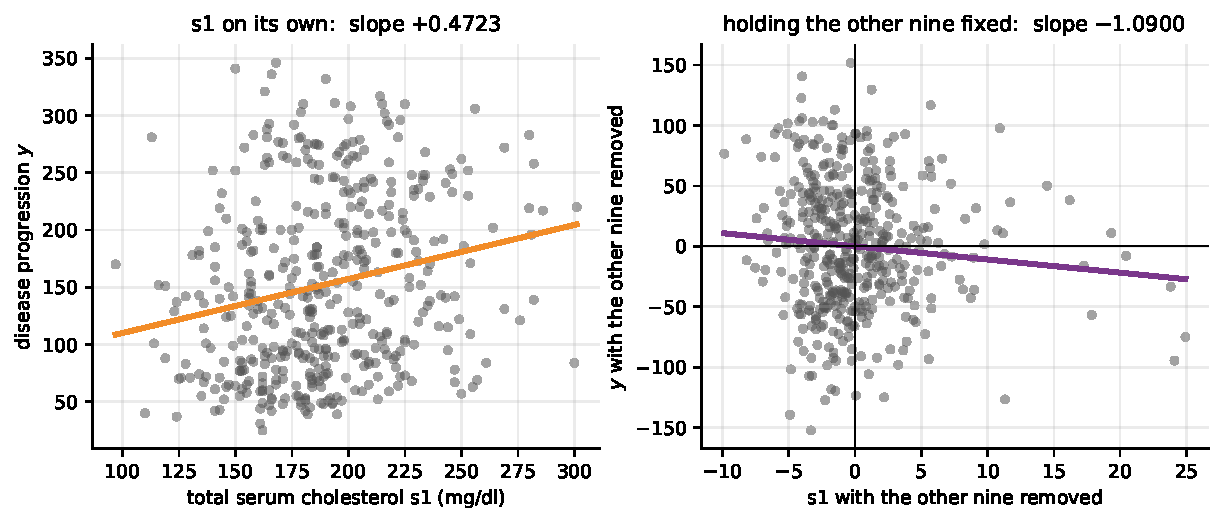
\includegraphics[width=0.86\textwidth]{signflip.pdf}
  \end{center}
  \begin{center}\small
    Left: raw \texttt{s1} against the target --- an upward cloud, slope
    $+0.4723$. Right: the \textbf{added-variable plot}. Both axes have had
    the other nine predictors regressed out, and what is left slopes
    \emph{down} at $-1.0900$. Same $442$ patients, same column, opposite
    conclusion.
  \end{center}
\end{frame}

\begin{frame}[fragile,shrink=8]{Where the difference went}
Fit $y$ on $x_1$ alone, and $y$ on $x_1$ and $x_2$. Then
$b^{\text{simple}}_1 = b_1 + b_2\,\delta$, where $\delta$ is the slope of
$x_2$ regressed on $x_1$.
\begin{outblk}
s1 (total cholesterol) alone            +0.4723
s1 with s5 (log triglycerides) added    -0.2418
s5 in that pair                         +91.7683
corr(s1, s5) +0.5155
   regress s5 on s1: delta = +0.007781
   -0.2418 + +91.7683 * +0.007781 = +0.4723   (simple slope +0.4723)
\end{outblk}
\onslide<2->
\begin{alertblock}{The simple slope was $91.77 \times 0.0078 = 0.714$ of borrowed effect}
  \footnotesize \texttt{s1} was carrying \texttt{s5}'s effect on its back,
  because the two correlate at $+0.52$. Remove the loan and what is left is
  $-0.24$. \textbf{Two predictors are enough to flip the sign; the other
  eight take it to $-1.09$.}
\end{alertblock}
\end{frame}

\begin{frame}[fragile,shrink=8]{Partial regression coefficients: the recipe}
The \textbf{partial regression coefficient} of $x_j$ is what you get from a
two-step construction that never mentions the other coefficients:
\begin{enumerate}\small
  \item Regress $x_j$ on all the \emph{other} predictors; keep the residual
    $\tilde x_j$ --- the part of $x_j$ nothing else explains.
  \item Regress $y$ on all the other predictors; keep the residual
    $\tilde y$.
  \item Regress $\tilde y$ on $\tilde x_j$. That single slope is $b_j$.
\end{enumerate}
\begin{outblk}
residual of s1 after regressing it on the other nine   sd 4.4979
residual of y  after regressing it on the other nine   sd 53.7607
slope of (y residual) on (s1 residual)  -1.0899963341
coefficient of s1 in the full model     -1.0899963341
difference 2.15e-14
\end{outblk}
\onslide<2->
\begin{center}\small
  This is the \textbf{Frisch--Waugh--Lovell} theorem, and it is the precise
  content of ``holding the others fixed''. The scatter of $\tilde y$ against
  $\tilde x_j$ is the \textbf{added-variable plot} --- the only honest
  two-dimensional picture of a multiple-regression coefficient.
\end{center}
\end{frame}

\begin{frame}[shrink=8]{Drawn: four added-variable plots}
  \begin{center}
    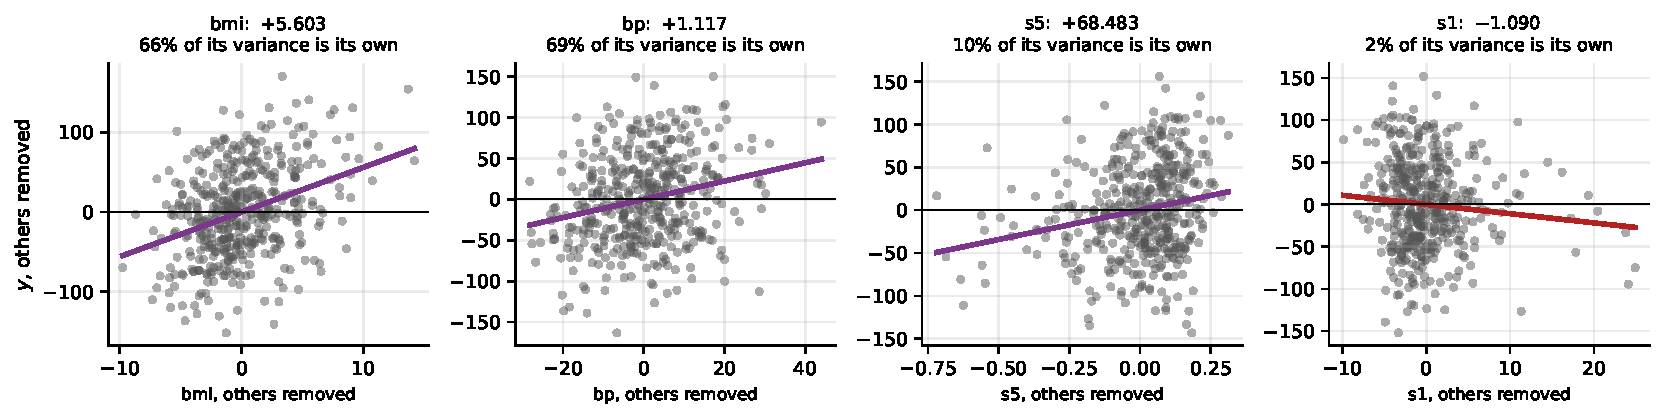
\includegraphics[width=0.98\textwidth]{avplot.pdf}
  \end{center}
  \begin{center}\small
    The slope of each cloud \emph{is} the coefficient in the ten-predictor
    model. Read the second line of each title: \textbf{$66\%$ of
    \texttt{bmi}'s variance survives the other nine, and only $1.7\%$ of
    \texttt{s1}'s does.} That is why \texttt{s1}'s cloud is narrow --- and
    why its coefficient will turn out to be untrustworthy.
  \end{center}
\end{frame}

% =====================================================================
\subsection[Standardized]{Standardized (beta) coefficients}
\label{sec:std}

\begin{frame}[shrink=6]{Raw coefficients cannot be compared}
  \begin{alertblock}{}
    \centering
    $b_j$ has units of $y$ per unit of $x_j$. Two coefficients with different
    denominators are \textbf{not the same kind of number}.
  \end{alertblock}
  \vspace{0.3em}
  \begin{columns}[T]
    \begin{column}{0.48\textwidth}
      \begin{block}{The fix}
        Standardise both sides before fitting, or equivalently rescale
        afterwards:
        \[ \beta^*_j = b_j\,\frac{s_j}{s_y} . \]
        \small $\beta^*_j$ is the change in $y$, \textbf{in standard
        deviations of $y$}, per one standard deviation of $x_j$. Unit-free,
        and therefore comparable.
      \end{block}
    \end{column}
    \begin{column}{0.48\textwidth}
      \begin{block}{Where the formula comes from}
        \small Replace $x_j$ by $(x_j - \bar x_j)/s_j$ and $y$ by
        $(y-\bar y)/s_y$. The design matrix column is divided by $s_j$, so
        its coefficient is multiplied by $s_j$; the target is divided by
        $s_y$, so every coefficient is divided by $s_y$.
      \end{block}
      \begin{alertblock}{One thing it does not fix}
        \small $\beta^*$ is still a \emph{conditional} quantity. Standardising
        makes the numbers comparable; it does not make them causal.
      \end{alertblock}
    \end{column}
  \end{columns}
\end{frame}

\begin{frame}[fragile,shrink=8]{Predict first \#2}
The full ten-predictor diabetes model, in original units. The largest raw
coefficient by a wide margin is \texttt{s5}, log serum triglycerides, at
$\mathbf{+68.48}$; \texttt{s1} is a mere $-1.09$, sixth of ten.

Their standard deviations: \texttt{s5} has $s_j = 0.52$ and \texttt{s1} has
$s_j = 34.61$.

\begin{center}
  \textbf{Which predictor has the largest \emph{standardized} coefficient,
  and where does \texttt{s1} land?}
\end{center}
\vspace{0.2em}
\onslide<2->
\begin{outblk}
feature    raw coef        sd      beta*   rank raw   rank beta*
s1           -1.0900   34.6081    -0.4893        6            1
s5          +68.4831    0.5224    +0.4640        1            2
bmi          +5.6030    4.4181    +0.3211        4            3
sex         -22.8596    0.4996    -0.1481        2            6
\end{outblk}
\onslide<3->
\begin{alertblock}{Sixth becomes first; second becomes sixth}
  \footnotesize \texttt{s1} moves from rank $6$ to rank $\mathbf{1}$ and
  \texttt{sex} from $2$ to $6$. \textbf{The raw ranking was a ranking of
  measurement units}: \texttt{s5} is a logarithm and spans half a unit,
  \texttt{s1} is in mg/dl and spans a hundred.
\end{alertblock}
\end{frame}

\begin{frame}[fragile,shrink=8]{And $\beta^*$ really is unit-free --- check it}
Record \texttt{bmi} in units of $10^{-4}\,\mathrm{kg/m^2}$ instead. Same data,
same model, same predictions.
\begin{outblk}
   bmi coefficient  +5.6030  (kg/m2)   +0.00056030  (1e-4 kg/m2)
   beta* for bmi    +0.321100  and  +0.321100   -- unchanged
\end{outblk}
\onslide<2->
\begin{outblk}
check against a regression on standardised columns: max diff 7.72e-15
\end{outblk}
\onslide<3->
\begin{columns}[T]
  \begin{column}{0.50\textwidth}
    \begin{block}{Two routes, one answer}
      \small Rescaling $b_j$ by $s_j/s_y$ gives \emph{exactly} what you get
      by putting \texttt{StandardScaler} in front of the regression. Use
      whichever is convenient.
    \end{block}
  \end{column}
  \begin{column}{0.46\textwidth}
    \begin{alertblock}{Do not over-read $\beta^*$ either}
      \small A large $\beta^*$ can still come from a collinear column with a
      wild coefficient, and $s_j$ depends on \emph{this} sample. It ranks;
      it does not adjudicate.
    \end{alertblock}
  \end{column}
\end{columns}
\end{frame}

\begin{frame}[shrink=8]{Drawn: two rankings of the same model}
  \begin{center}
    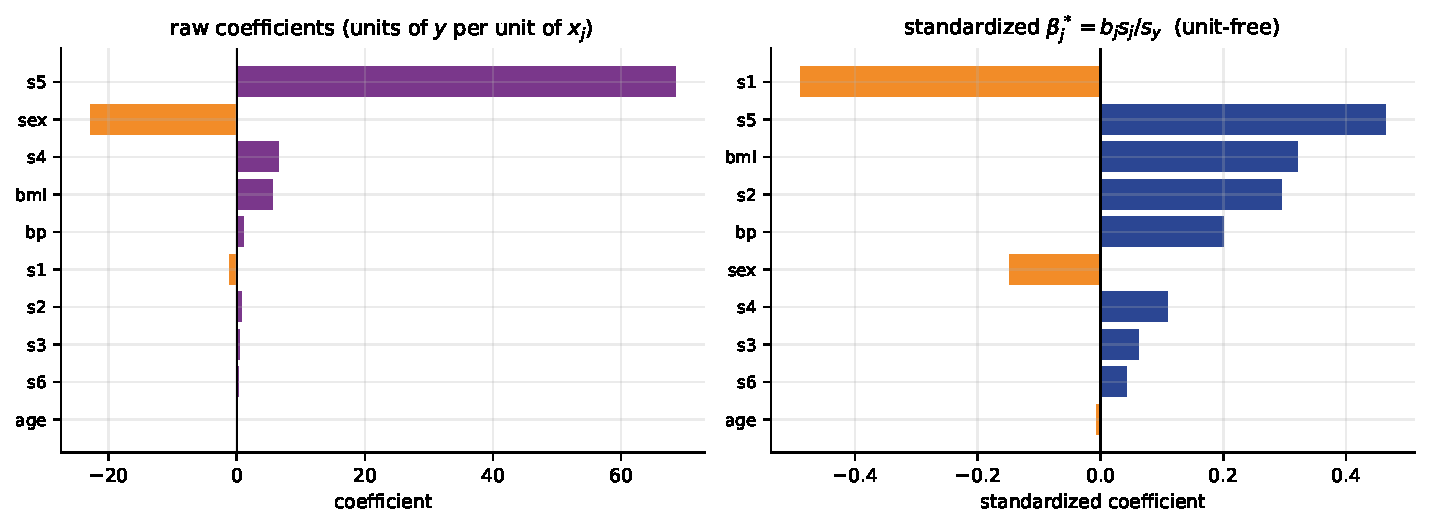
\includegraphics[width=0.86\textwidth]{stdcoef.pdf}
  \end{center}
  \begin{center}\small
    Left: raw coefficients, sorted. One bar is fifty times the others and it
    tells you nothing except that \texttt{s5} is measured in small numbers.
    Right: the same fit, standardised. \textbf{Five predictors now sit within
    a factor of two of each other, and \texttt{s1} has come first.}
  \end{center}
\end{frame}

% =====================================================================
\section[VIF]{Multicollinearity}
\label{sec:mc}

\begin{frame}[shrink=6]{Near-dependence: the matrix is invertible, barely}
  \begin{block}{The quantity that matters}
    Let $R_j^2$ be the $R^2$ from regressing $x_j$ on \emph{all the other
    predictors}. Then
    \[
      \mathrm{VIF}_j = \frac{1}{1 - R_j^2},
      \qquad
      \operatorname{Var}(\hat\beta_j) =
      \frac{\sigma^2}{(n-1)s_j^2}\cdot \mathrm{VIF}_j .
    \]
    The \textbf{variance inflation factor} is the factor by which collinearity
    multiplies the variance of $\hat\beta_j$. Standard errors are multiplied
    by $\sqrt{\mathrm{VIF}_j}$.
  \end{block}
  \begin{columns}[T]
    \begin{column}{0.48\textwidth}
      \begin{exampleblock}{Reading it}
        \small $R_j^2 = 0 \Rightarrow \mathrm{VIF} = 1$: no inflation at all.
        $R_j^2 = 0.9 \Rightarrow \mathrm{VIF} = 10$. $R_j^2 = 0.99
        \Rightarrow \mathrm{VIF} = 100$, so ten times the standard error.
      \end{exampleblock}
    \end{column}
    \begin{column}{0.48\textwidth}
      \begin{alertblock}{Rules of thumb, and their status}
        \small $\mathrm{VIF} > 5$ deserves a look, $> 10$ is usually a
        problem. They are conventions, not theorems --- what matters is
        whether the coefficient you intend to \emph{interpret} is one of the
        inflated ones.
      \end{alertblock}
    \end{column}
  \end{columns}
\end{frame}

\begin{frame}[fragile,shrink=8]{VIF on the diabetes table}
\begin{lstlisting}
def vif(A):
    return np.array([1 / (1 - LinearRegression()
        .fit(np.delete(A, j, 1), A[:, j])
        .score(np.delete(A, j, 1), A[:, j])) for j in range(A.shape[1])])
\end{lstlisting}
\begin{outblk}
feature      R2_j      VIF   sqrt(VIF)
s1         0.9831    59.20     7.69
s2         0.9745    39.19     6.26
s3         0.9351    15.40     3.92
s5         0.9008    10.08     3.17
s4         0.8875     8.89     2.98
bmi        0.3375     1.51     1.23
s6         0.3264     1.48     1.22
bp         0.3148     1.46     1.21
sex        0.2176     1.28     1.13
age        0.1785     1.22     1.10
\end{outblk}
\onslide<2->
\begin{center}\small
  The five serum measurements are five views of one blood sample:
  $\texttt{s4} = \texttt{s1}/\texttt{s3}$ by definition, and \texttt{s2} is a
  component of \texttt{s1}. \textbf{$98.3\%$ of \texttt{s1} is predictable
  from the other nine columns}, so its standard error is $7.7$ times what it
  would be if the columns were orthogonal.
\end{center}
\end{frame}

\begin{frame}[shrink=8]{Drawn: variance inflation, measured and plotted}
  \begin{center}
    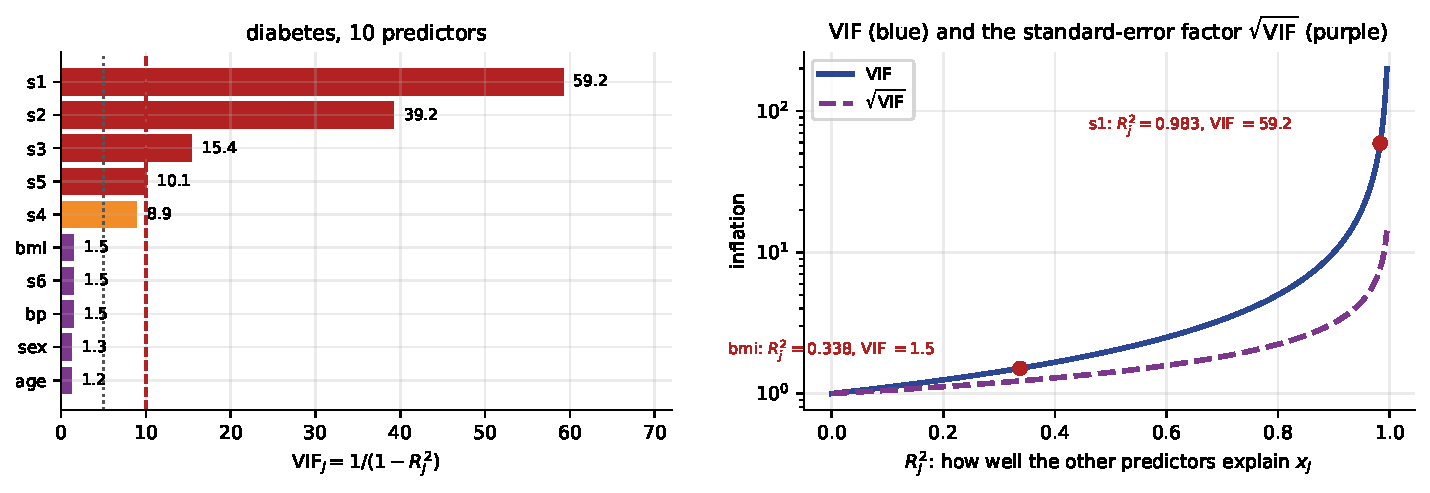
\includegraphics[width=0.90\textwidth]{vif.pdf}
  \end{center}
  \begin{center}\small
    Left: the ten VIFs, with the conventional thresholds at $5$ and $10$.
    Right: the curve $1/(1-R_j^2)$ on a log axis. \textbf{It is flat until
    $R_j^2 \approx 0.8$ and then vertical} --- which is why collinearity
    tends to arrive suddenly rather than gradually.
  \end{center}
\end{frame}

\begin{frame}[fragile,shrink=8]{Predict first \#3}
Resample the $442$ patients with replacement, refit, and repeat $2000$ times.
Every resample is a plausible alternative dataset from the same population.

The fitted coefficient of \texttt{s1} is $-1.090$, and of \texttt{bmi} is
$+5.603$.

\begin{center}
  \textbf{How wide are the two bootstrap distributions, and does either of
  them cross zero?}
\end{center}
\vspace{0.2em}
\onslide<2->
\begin{outblk}
feature    coef    boot sd    2.5%      97.5%     VIF   sign flips
s1         -1.090    0.565    -2.093    +0.113    59.2      3.8%
s2         +0.746    0.512    -0.325    +1.634    39.2      8.6%
s5        +68.483   14.982   +39.101   +97.225    10.1      0.0%
bmi        +5.603    0.721    +4.159    +6.996     1.5      0.0%
\end{outblk}
\onslide<3->
\begin{alertblock}{\texttt{s2} changes sign in one resample out of twelve}
  \footnotesize \texttt{bmi}'s interval is $[+4.16, +7.00]$ --- never near
  zero, VIF $1.5$. \texttt{s1}'s is $[-2.10, +0.06]$ and \texttt{s2}'s is
  $[-0.30, +1.69]$: \textbf{both straddle zero}, and neither sign is
  established by $442$ patients. \textbf{The correlation between the
  bootstrap \texttt{s1} and \texttt{s2} coefficients is $-0.964$.}
\end{alertblock}
\end{frame}

\begin{frame}[shrink=8]{Drawn: what the bootstrap sees}
  \begin{center}
    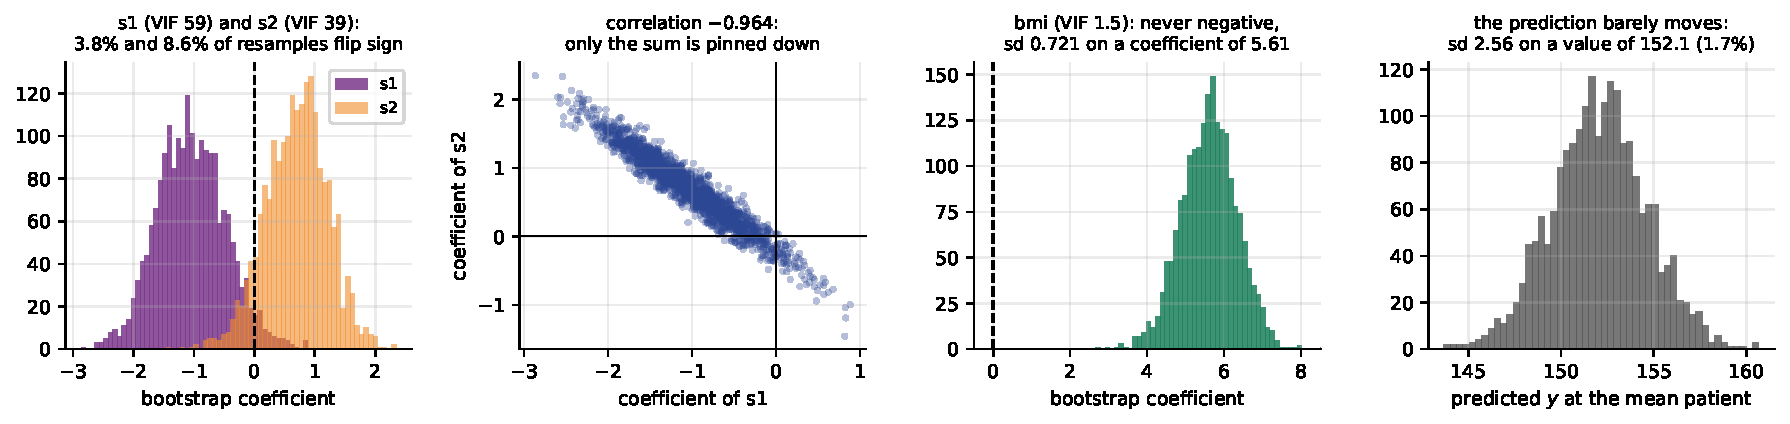
\includegraphics[width=0.98\textwidth]{boot.pdf}
  \end{center}
  \begin{center}\small
    Panels 1 and 2: the \texttt{s1} and \texttt{s2} coefficients slide along
    a line of slope $-1$ --- \textbf{their sum is pinned down and the split
    between them is not}. Panel 3: \texttt{bmi}, VIF $1.5$, never negative.
    Panel 4: \textbf{the prediction at the mean patient has a spread of
    $1.7\%$}, while the coefficients feeding it are barely determined.
  \end{center}
\end{frame}

\begin{frame}[fragile,shrink=8]{Predicting is fine. Explaining is not.}
Two predictors correlated at $0.9986$; the truth is $y = 3x_1 + 2x_2 +
\varepsilon$. Fit on the first hundred rows, then on the second hundred.
\begin{outblk}
corr(a, b) 0.9986    true coefficients 3.0 and 2.0     VIF [351.6 351.6]
first half   a   +2.553  b   +2.460   sum  +5.012   test R2 +0.9895
second half  a   +2.208  b   +2.848   sum  +5.056   test R2 +0.9895
the two coefficient vectors differ by 0.39, their sum by 0.044
\end{outblk}
\onslide<2->
\begin{outblk}
cross-validated R2, all 10 features        +0.4892
cross-validated R2, s1 dropped             +0.4867
cross-validated R2, s1 and s2 both dropped +0.4867
\end{outblk}
\onslide<3->
\begin{alertblock}{One model says $b_2 = +1.91$, the other says $-0.60$}
  \footnotesize Both score $R^2 = 0.989$ on the same test data. Dropping the
  worst two diabetes predictors costs $0.0025$ of cross-validated $R^2$.
  \textbf{Multicollinearity is a disease of the coefficients, not of the
  predictions.} If you only need $\hat y$, you may ignore it. If anyone will
  read a coefficient, you may not.
\end{alertblock}
\end{frame}

\begin{frame}[shrink=8]{Drawn: a valley, not a bowl}
  \begin{center}
    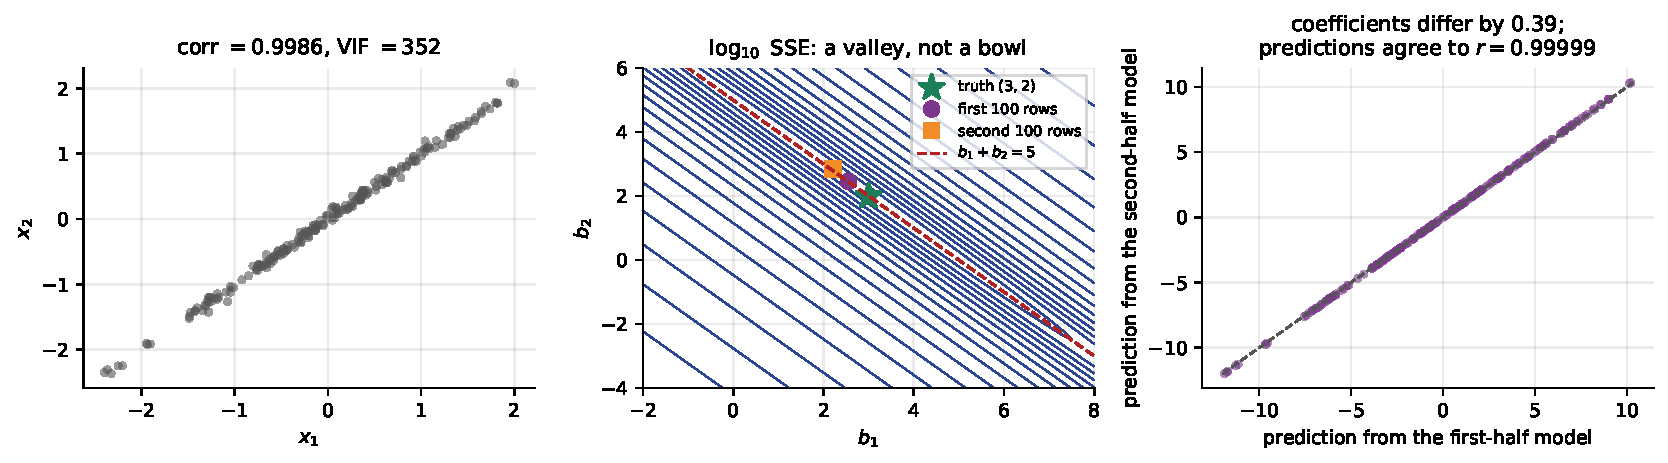
\includegraphics[width=0.98\textwidth]{collinear.pdf}
  \end{center}
  \begin{center}\small
    Middle panel: the SSE contours are a long trench along $b_1 + b_2 = 5$.
    Any point in the trench fits almost equally well, and which one you land
    on is decided by noise --- purple and orange are two halves of the same
    dataset. Right: \textbf{their predictions agree to $r = 0.99999$.}
  \end{center}
\end{frame}

\begin{frame}[shrink=6]{What to do about collinearity}
  \begin{center}\small
  \begin{tabular}{@{}lp{4.6cm}p{4.4cm}@{}}
    \toprule
    & \textbf{What it does} & \textbf{Cost}\\
    \midrule
    \textbf{Nothing} & fine if you only predict &
      no coefficient may be interpreted\\[3pt]
    \textbf{Drop a column} & removes the redundancy &
      the survivor now carries both effects; the choice is scientific, not
      statistical\\[3pt]
    \textbf{Combine columns} & a sum, a ratio, an index &
      you must be able to name the combination\\[3pt]
    \textbf{Ridge / lasso} & $\Xt X + \lambda I$ is always invertible &
      biased coefficients, chosen by cross-validation --- \emph{next
      lecture}\\[3pt]
    \textbf{Collect more data} & shrinks every standard error &
      does not help if the columns are collinear \emph{by definition}\\
    \bottomrule
  \end{tabular}
  \end{center}
  \begin{alertblock}{Measured, on diabetes}
    \small Least squares on standardised columns gives \texttt{s1} $= -37.68$
    and \texttt{s2} $= +22.68$; ridge at $\alpha = 1$ gives $-30.09$ and
    $+16.65$, and cross-validated $R^2$ moves from $0.4892$ to $0.4896$.
    \textbf{Same predictions, calmer coefficients.}
  \end{alertblock}
\end{frame}

% =====================================================================
\section[Missing]{Missing data in a regression}
\label{sec:missing}

\begin{frame}[shrink=6]{Why missing data is worse in multiple regression}
  \begin{alertblock}{}
    \centering
    Least squares needs a \textbf{complete row}. One missing cell in one
    column removes the whole patient.
  \end{alertblock}
  \vspace{0.3em}
  \begin{columns}[T]
    \begin{column}{0.48\textwidth}
      \begin{block}{The arithmetic of complete cases}
        With $d$ columns each missing independently at rate $p$, a row
        survives with probability $(1-p)^d$.
        \begin{center}\small
        \begin{tabular}{@{}rrr@{}}
          \toprule
          $p$ & rows kept of $309$ & \%\\
          \midrule
          $0.01$ & $279$ & $90.4$\\
          $0.05$ & $185$ & $59.9$\\
          $0.10$ & $108$ & $34.9$\\
          $0.25$ & $\phantom{00}9$ & $\phantom{0}5.6$\\
          \bottomrule
        \end{tabular}
        \end{center}
      \end{block}
    \end{column}
    \begin{column}{0.48\textwidth}
      \begin{block}{Carried over from Lecture 5}
        \small \textbf{MCAR} --- complete cases are a fair sample; you lose
        power, not correctness. \textbf{MAR} --- complete cases are biased,
        but the observed columns can undo it. \textbf{MNAR} --- the
        missingness depends on the value itself and no amount of arithmetic
        repairs it.
      \end{block}
      \begin{alertblock}{The multiple-regression twist}
        \small $10\%$ per cell sounds small. Across ten predictors it deletes
        \textbf{two thirds of your patients}, and it does so silently.
      \end{alertblock}
    \end{column}
  \end{columns}
\end{frame}

\begin{frame}[fragile,shrink=8]{Measured: five ways to handle it}
$309$ training rows, $10$ predictors, MCAR missingness, evaluated on a
held-out third that is complete.
\begin{outblk}
no missingness at all                test R2 +0.3929

MCAR at 10%: cells missing 10.4%, complete rows 103 of 309 (33.3%)
   listwise deletion            103 rows   test R2 +0.3231
   mean imputation              309 rows   test R2 +0.3875
   mean + missing indicators    309 rows   test R2 +0.3657
   IterativeImputer (MICE)      309 rows   test R2 +0.3871
\end{outblk}
\onslide<2->
\begin{outblk}
MCAR at 25%: cells missing 25.2%, complete rows 13 of 309 (4.2%)
   listwise deletion             13 rows   test R2 -2.1451
   mean imputation              309 rows   test R2 +0.4048
   IterativeImputer (MICE)      309 rows   test R2 +0.4038
\end{outblk}
\onslide<3->
\begin{alertblock}{$-2.15$: worse than predicting the mean of $y$ every time}
  \footnotesize At $25\%$, listwise deletion leaves $13$ rows for $11$
  parameters and the model is nonsense. \textbf{Mean imputation, the crudest
  method there is, gives $+0.405$ on the same data}, and MICE $+0.404$,
  against a no-missingness $+0.393$. Those last two differ by $0.001$:
  \textbf{do not rank them}. The measurable effect is that deleting rows
  costs $2.54$ and imputing costs nothing.
\end{alertblock}
\end{frame}

\begin{frame}[shrink=8]{Drawn: the cliff, and what climbs it}
  \begin{center}
    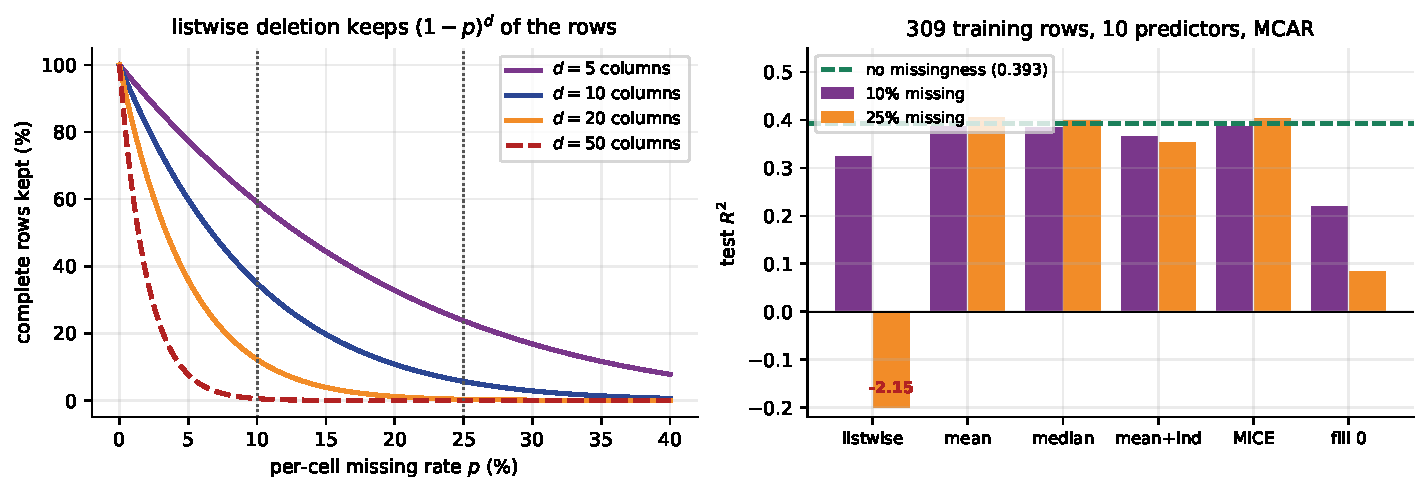
\includegraphics[width=0.88\textwidth]{missing.pdf}
  \end{center}
  \begin{center}\small
    Left: $(1-p)^d$ for four widths of table. At $d = 50$ a $5\%$ cell rate
    keeps a fifth of your rows. Right: the five strategies at two rates. The
    listwise bar at $25\%$ is off the bottom of the axis at $-3.26$;
    \textbf{filling with $0$ is the other bad answer}, because a patient with
    age $0$ and blood pressure $0$ is a claim, not a gap.
  \end{center}
\end{frame}

\begin{frame}[fragile,shrink=8]{The imputer is a learned step}
\begin{lstlisting}
# wrong: the column means are computed from every row, including test rows
X_filled = SimpleImputer().fit_transform(X)
cross_val_score(LinearRegression(), X_filled, y, cv=5)

# right: refitted on four fifths of the data inside every fold
cross_val_score(Pipeline([("imp", SimpleImputer()),
                          ("lr",  LinearRegression())]), X, y, cv=5)
\end{lstlisting}
\begin{outblk}
25% MCAR on all 442 rows, 5-fold cross-validation
   mean    impute-then-split +0.4114   inside the Pipeline +0.4112   difference +0.0002
   MICE    impute-then-split +0.4434   inside the Pipeline +0.4392   difference +0.0042
\end{outblk}
\onslide<2->
\begin{alertblock}{Report this honestly: the leak here is tiny}
  \footnotesize $+0.0002$ and $+0.0042$. An imputer never looks at $y$, so
  there is very little for it to absorb --- exactly the argument Lecture~6
  made for PCA. \textbf{Put it in the \texttt{Pipeline} anyway}: it costs
  nothing, and a target-aware imputer on a small test set is a different
  story.
\end{alertblock}
\end{frame}

% =====================================================================
\section[Checks]{Model validation}
\label{sec:valid}

\begin{frame}[shrink=6]{Three different questions, three different checks}
  \begin{center}\small
  \begin{tabular}{@{}p{3.6cm}p{4.2cm}p{4.2cm}@{}}
    \toprule
    \textbf{Question} & \textbf{Check} & \textbf{What failure looks like}\\
    \midrule
    Are the \emph{assumptions} met? &
      residual plots, Q--Q plot, scale--location &
      curvature, a fan, heavy tails\\[4pt]
    Does it \emph{generalise}? &
      train against test, or cross-validation &
      a large gap between the two\\[4pt]
    Is the extra column \emph{earning its place}? &
      adjusted $R^2$, held-out $R^2$, an $F$ test &
      $R^2$ up, adjusted $R^2$ and test $R^2$ down\\
    \bottomrule
  \end{tabular}
  \end{center}
  \vspace{0.3em}
  \begin{alertblock}{And remember what is guaranteed}
    \small $\sum e_i = 0$ and $\operatorname{corr}(e, \hat y) = 0$ are forced
    by the normal equations. Measured on diabetes: residual mean
    $-8.1\times10^{-14}$, correlation with fitted $5.4\times10^{-16}$.
    \textbf{Neither is evidence of anything.}
  \end{alertblock}
\end{frame}

\begin{frame}[fragile,shrink=8]{Residual diagnostics on the diabetes fit}
\begin{outblk}
diabetes, 10 features, 309 training rows
   train R2 +0.5539   test R2 +0.3929
   train RMSE 52.954  test RMSE 55.652
   Shapiro-Wilk on the residuals: W 0.9959, p 0.6100
   corr(|residual|, fitted) +0.2079, p 0.0002
\end{outblk}
\onslide<2->
\begin{columns}[T]
  \begin{column}{0.50\textwidth}
    \begin{block}{What passed}
      \small Normality: $p = 0.11$, no evidence against it. Train and test
      RMSE agree to within about $5\%$, so no overfitting worth worrying
      about at $309 \times 10$.
    \end{block}
  \end{column}
  \begin{column}{0.46\textwidth}
    \begin{alertblock}{What did not}
      \small $|e|$ rises with $\hat y$ ($p = 0.0002$): mild
      \textbf{heteroscedasticity}. The coefficients are still unbiased; the
      standard errors are not, and prediction intervals will be too narrow
      at the top end.
    \end{alertblock}
  \end{column}
\end{columns}
\end{frame}

\begin{frame}[shrink=8]{Drawn: four diagnostic panels}
  \begin{center}
    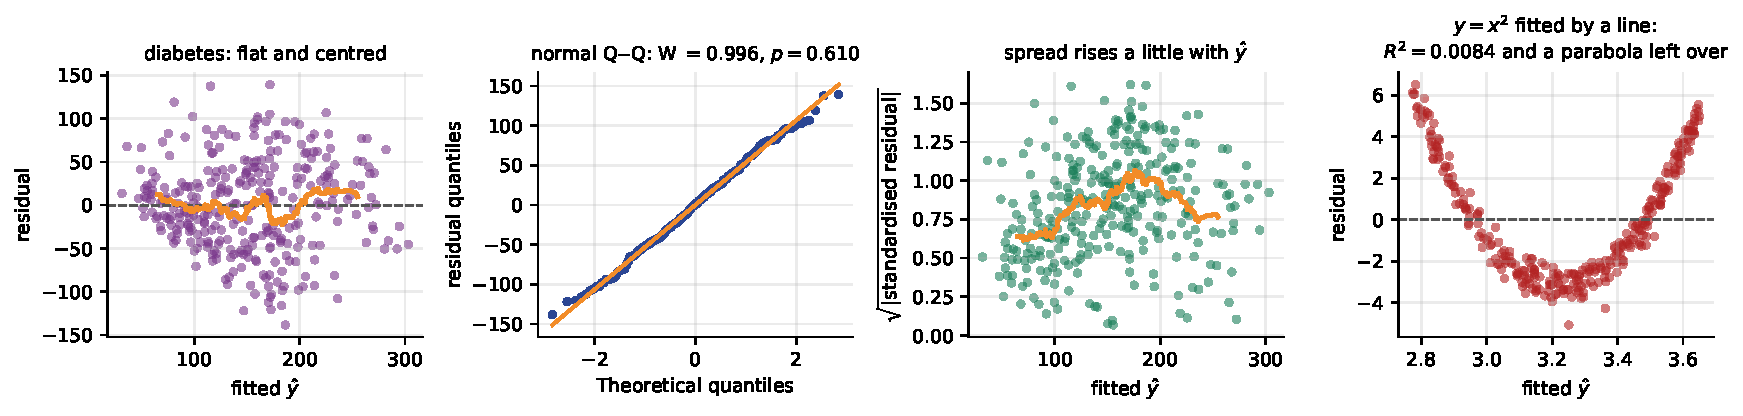
\includegraphics[width=0.98\textwidth]{resid.pdf}
  \end{center}
  \begin{center}\small
    The first three are the diabetes fit: flat, straight, slightly fanning.
    \textbf{The fourth is the point of the slide} --- $y = x^2$ fitted by a
    straight line. $R^2 = 0.0000$, the residual mean is zero and the residual
    correlation with $\hat y$ is zero, and the residual plot is a parabola.
    \textbf{Look at the picture, not only at the summary.}
  \end{center}
\end{frame}

\begin{frame}[fragile,shrink=8]{Predict first \#4}
$80$ training rows of diabetes, all $10$ real predictors, train $R^2 =
0.5911$. Now append $k$ columns of $\mathcal{N}(0,1)$ noise, independent of
everything, and refit.

\begin{center}
  \textbf{What happens to the training $R^2$? To the adjusted $R^2$?
  To the $R^2$ on held-out rows?}
\end{center}
\vspace{0.2em}
\onslide<2->
\begin{outblk}
 junk k      p   train R2   adj R2    test R2
      0     10     0.5911   0.5318     0.2488
      1     11     0.5992   0.5344     0.2295
      5     15     0.6183   0.5289     0.1719
     10     20     0.6407   0.5188     0.1340
     20     30     0.6935   0.5059    -0.0794
\end{outblk}
\onslide<3->
\begin{alertblock}{$R^2$ rose at every one of the eight steps. It always does.}
  \footnotesize Adding a column can never increase SSE --- the old solution
  is still available with a coefficient of zero --- so $R^2$ is
  \textbf{monotone non-decreasing in $p$, whatever the column contains}.
  Adjusted $R^2$ was \textbf{fooled by the first junk column} and peaked
  there rather than at none, and test $R^2$ fell at \textbf{seven of eight}
  steps, from $+0.249$ to $\mathbf{-0.079}$ --- past zero.
\end{alertblock}
\end{frame}

\begin{frame}[shrink=6]{Adjusted $R^2$: the correction and its limits}
  \[
    R^2 = 1 - \frac{\mathrm{SSE}}{\mathrm{SST}},
    \qquad
    R^2_{\text{adj}} = 1 - \frac{\mathrm{SSE}/(n-p-1)}
                                {\mathrm{SST}/(n-1)}
                     = 1 - (1-R^2)\,\frac{n-1}{n-p-1}.
  \]
  \begin{columns}[T]
    \begin{column}{0.48\textwidth}
      \begin{block}{What the correction does}
        \small $R^2$ compares two sums; $R^2_{\text{adj}}$ compares two
        \emph{mean} squares. A useless column reduces SSE a little and the
        denominator $n-p-1$ a lot, so the ratio rises and
        $R^2_{\text{adj}}$ falls. \textbf{It can go negative.}
      \end{block}
    \end{column}
    \begin{column}{0.48\textwidth}
      \begin{alertblock}{Where it stops being useful}
        \small As $p \to n-1$ the factor $(n-1)/(n-p-1)$ explodes and the
        statistic becomes noise. Measured: at $k=60$ junk columns with $80$
        rows, train $R^2 = 0.976$, test $R^2 = -7.35$, and
        $R^2_{\text{adj}}$ reads a cheerful $0.786$.
      \end{alertblock}
    \end{column}
  \end{columns}
  \vspace{0.2em}
  \begin{center}\small
    \textbf{Adjusted $R^2$ is a warning light, not a model-selection
    criterion.} Held-out error is the criterion. On the five flats:
    $R^2 = 0.8507$ against $R^2_{\text{adj}} = 0.7015$, because two
    parameters on five rows is a lot of parameters.
  \end{center}
\end{frame}

\begin{frame}[shrink=8]{Drawn: the two curves separating}
  \begin{center}
    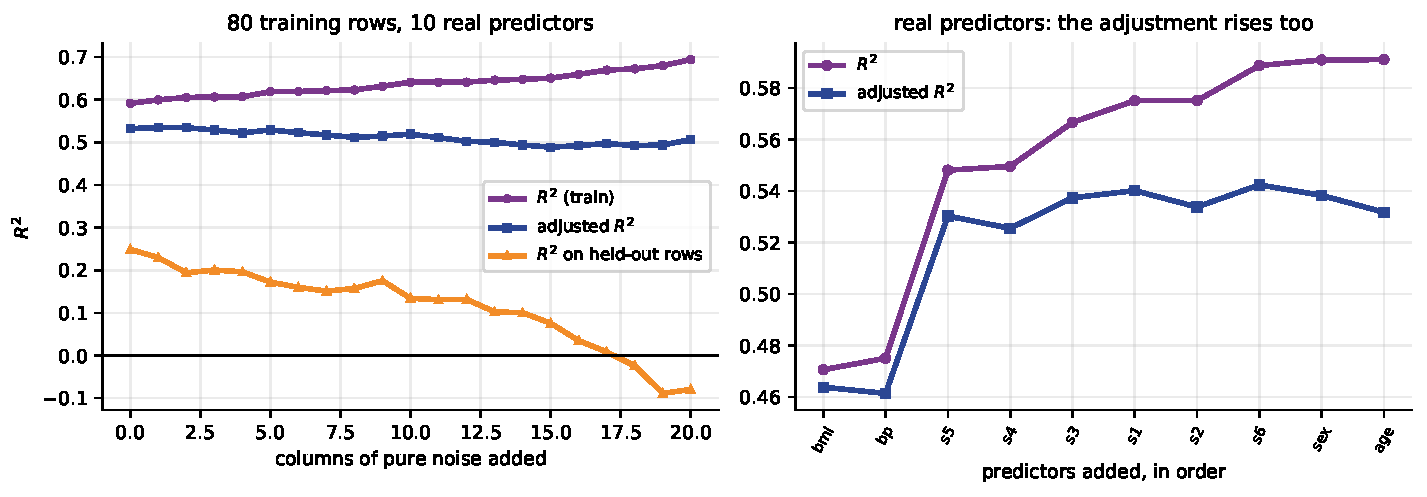
\includegraphics[width=0.86\textwidth]{adjr2.pdf}
  \end{center}
  \begin{center}\small
    Left: purple ($R^2$) only ever rises; blue (adjusted) drifts down; orange
    (held-out) falls off a cliff. Right: the same three-column arithmetic
    when the added predictors are \emph{real} --- both curves rise together,
    and the dip at \texttt{s1} and \texttt{s2} is the adjustment noticing
    that those two columns are nearly redundant.
  \end{center}
\end{frame}

\begin{frame}[fragile,shrink=6]{The whole thing, as one object}
\begin{lstlisting}
pipe = Pipeline([
    ("imp",   SimpleImputer(strategy="median")),
    ("scale", StandardScaler()),        # so the coefficients are beta*
    ("model", LinearRegression()),
])
cross_val_score(pipe, X, y, cv=KFold(5, shuffle=True, random_state=0))
\end{lstlisting}
\begin{outblk}
impute -> standardise -> least squares, 5-fold on the 10%-missing table
   fold R2 [0.2632 0.3567 0.5213 0.3747 0.5293]
   mean +0.4090  sd 0.1143
   for comparison, the same pipeline on the complete table: +0.4892
\end{outblk}
\onslide<2->
\begin{center}\small
  The column medians and the column means and standard deviations are
  recomputed inside every fold. \textbf{And read the fold-to-fold spread:
  $0.28$ to $0.49$.} A single train/test split of $442$ patients would have
  reported any number in that range with equal confidence.
\end{center}
\end{frame}

% =====================================================================
\section{Summary}
\label{sec:summary}

\begin{frame}[shrink=16]{Summary --- twelve lines}
  \begin{enumerate}\small
    \item $y = X\beta + \varepsilon$. Differentiating
      $(y-Xb)^{\!\top}(y-Xb)$ gives $\nabla S = -2\Xt y + 2\Xt X b$, so
      $\Xt X\hat\beta = \Xt y$ and $\hat\beta = (\Xt X)^{-1}\Xt y$. The
      Hessian $2\Xt X$ is positive semi-definite, so the stationary point is
      a global minimum.
    \item $\Xt X$ is invertible exactly when $X$ has full column rank,
      because $\operatorname{null}(\Xt X) = \operatorname{null}(X)$. Perfect
      collinearity and $p+1 > n$ are the two ways to lose it.
    \item Five flats, integer arithmetic: $\det \Xt X = 60$,
      $\hat\beta = (2, -1, 4)$, residuals $(-1, 1, 0, 1, -1)$,
      $\Xt e = 0$, $R^2 = 0.8507$, $R^2_{\text{adj}} = 0.7015$. Identical to
      \texttt{LinearRegression} at $8.6\times10^{-14}$.
    \item $b_j$ means ``holding the others fixed''. The bedroom coefficient
      is $-1$ because flats B and D have the same area.
    \item \textbf{\texttt{s1} has slope $+0.4723$ alone and $-1.0900$ with
      nine others in the model}, and four of the ten diabetes predictors
      change sign that way.
    \item The omitted-variable identity accounts for it exactly:
      $-0.2418 + 91.7683 \times 0.007781 = +0.4723$.
    \item Frisch--Waugh--Lovell: residualise both sides on the other
      predictors and the single slope is $b_j$, to $2\times10^{-14}$. That
      scatter is the added-variable plot.
    \item Standardizing changes the ranking: \texttt{s1} moves from sixth by
      raw magnitude to \textbf{first} by $\beta^*$, and $\beta^*$ is
      unchanged when \texttt{bmi} is rescaled by $10^{4}$.
    \item $\mathrm{VIF}_j = 1/(1-R_j^2)$. Four of ten exceed $10$;
      \texttt{s1} reaches $59.2$, so its standard error is $7.7\times$
      inflated.
    \item $2000$ bootstrap resamples: \texttt{s1} and \texttt{s2} straddle
      zero and correlate at $-0.964$, while the prediction at the mean
      patient has a spread of $1.7\%$. On a collinear pair whose truth was
      $(3,2)$, two halves gave $(+2.55,+2.46)$ and $(+2.21,+2.85)$ --- both
      wrong --- with test $R^2 = 0.9895$ both times.
      \textbf{Collinearity breaks explanation, not prediction.}
    \item $10\%$ missing cells across $10$ columns deletes two thirds of the
      rows; at $25\%$ listwise deletion scores $\mathbf{-2.15}$ while mean
      imputation scores $+0.405$ and MICE $+0.404$.
    \item $R^2$ rose at all eight steps as noise columns were added; adjusted
      $R^2$ was fooled by the first one, and held-out $R^2$ fell from
      $+0.249$ to $-0.079$. \textbf{Only the held-out number is a criterion.}
  \end{enumerate}
\end{frame}

\begin{frame}[shrink=3]{Before the next lecture}
  \begin{columns}[T]
    \begin{column}{0.48\textwidth}
      \begin{block}{Read}
        \texttt{notes.pdf} --- the full matrix derivation with every step,
        the Frisch--Waugh--Lovell proof, the variance formula behind VIF, and
        \textbf{10 practice questions with worked solutions}.
      \end{block}
      \begin{block}{Do}
        Questions 2, 5 and 9. Question 2 is a $3\times3$ inverse and
        $\hat\beta$ by hand; question 9 is a report you will be asked to
        review for real.
      \end{block}
    \end{column}
    \begin{column}{0.48\textwidth}
      \begin{exampleblock}{Next: ridge and lasso}
        Regularisation replaces $\Xt X$ by $\Xt X + \lambda I$, which is
        invertible for every $\lambda > 0$. \textbf{Every failure in this
        lecture is a reason that lecture exists.}
      \end{exampleblock}
      \begin{alertblock}{A habit to start now}
        Before you interpret any coefficient, print the VIFs and bootstrap
        the fit. If the interval straddles zero, say so --- do not report a
        sign the data has not established.
      \end{alertblock}
    \end{column}
  \end{columns}
  \begin{center}
    \small Materials: \texttt{\AMLRepoURL}
  \end{center}
  \slidesources{\AMLUnitVSources}
\end{frame}

\end{document}
